\section{Les limites d'ADTool}
	\label{sec:adtool}

	ADTool permet de construire un ADTree sans difficulté. Le logiciel offre la possibilité de créer de nouveaux nœuds, d'éditer leur label et de leur ajouter des fils de façon intuitive et simple. Le choix des opérateurs entre ces nœuds --- conjonction ou disjonction ---  se fait sans effort, et la mise en place de défenses est également réalisable très facilement. 
	
	\begin{figure}[h]
            \centering
            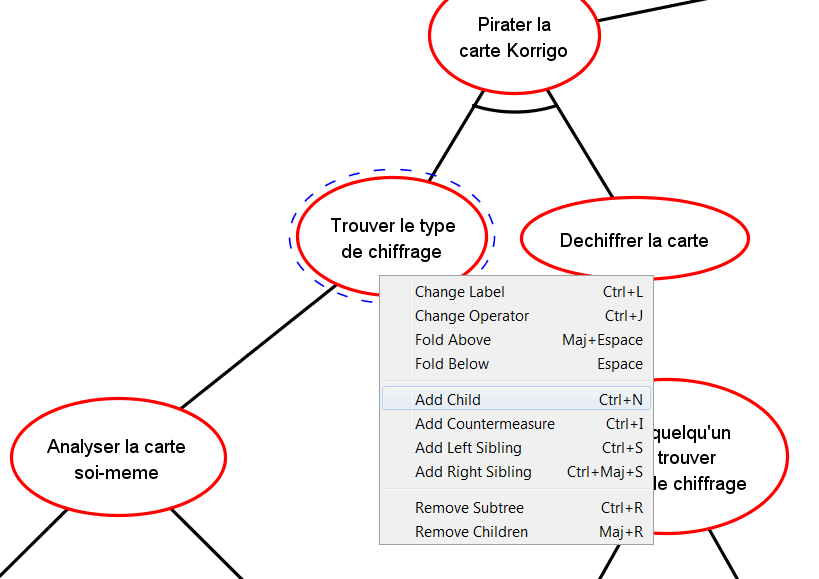
\includegraphics[width=1\textwidth]{figure/adtool_add_child.png}
            \caption{La création d'un arbre est simplifiée par des fonctions accessibles facilement.}
            \label{fig:arbre_exemple_1}
    \end{figure}
	
	
	Une fois l'arbre établi, il est possible d'ajouter des valuations à chaque feuille\footnote{Une feuille est un nœud n'ayant aucun fils.} de l'arbre selon un paramètre de base, tel que leur coût financier, leur probabilité de réussite, etc. (voir Section \ref{sec::mouloud}). ADTool se charge ensuite de propager les valuations aux nœuds-père de façon récursive, jusqu'à la racine.
	
	\begin{figure}[h]
            \centering
            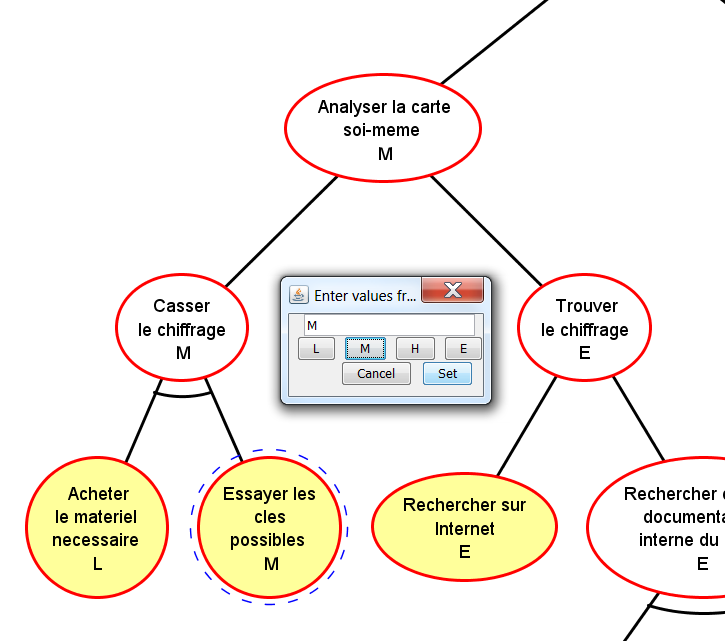
\includegraphics[width=1\textwidth]{figure/adtool_add_values.png}
            \caption{L'ajout de valuation aux feuilles est simple. Ces valuations se propagent ensuite récursivement aux nœuds-pères.}
            \label{fig:arbre_exemple_1}
    \end{figure}
	
	Dans l'exemple de la {\sc Figure} \ref{fig:arbre_exemple_1}, chaque noeud possède une valuation selon le paramètre de base \og difficulté de réalisation \fg{}. Cette valuation peut prendre la valeur L, M, H ou E ((\emph{Low}, \emph{Medium}, \emph{High} ou \emph{Extrem} --- voir Section \ref{sec::mouloud} pour plus de détails). En éditant la difficulté de réalisation de la feuille \og essayer les clés de cryptage possible \fg{}  à \emph{Medium}, la valuation du nœud-père \og casser le cryptage \fg{} est recalculée pour prendre la valeur \emph{Medium} : en effet, la difficulté de ce nœud conjonctif correspond à la difficulté la plus élevée de ses fils. Puis, à son tour, la valuation du père de ce nœud-père est recalculée à \emph{Middle}, car, étant un nœud disjonctif, sa difficulté de réalisation correspond à la difficulté la plus faible de ses fils.
	
	L'utilisateur n'a donc pas de calcul à faire lui-même pour obtenir la valuation de la racine de son arbre, c'est-à-dire la valuation de son objectif final. Cependant, l'analyse de l'arbre ainsi construit ne va pas plus loin. En effet, les valuations ne peuvent déjà se faire que selon un seul paramètre : il n'est pas possible de prendre en compte la \og difficulté \fg{} ET le \og temps nécessaire \fg{} à la réalisation d'un nœud, par exemple. Ceci est contraignant, car il est difficile de séparer ces deux notions : par exemple, le noeud \og essayer les clés de cryptage possible \fg{} est très facile à effectuer (il suffit de taper les clés une-à-une jusqu'à trouver la bonne), mais le temps nécessaire pour effectivement essayer chaque clé est colossal. ADTool ne permet donc pas de combiner plusieurs valuations pour obtenir une vision plus complète de l'arbre.
	
	 De plus, ADTool ne précise pas non plus d'où provient la valuation d'un nœud : par conséquent, pour la racine de l'arbre, l'utilisateur n'a aucun moyen de connaitre l'origine de sa valuation. Le \og meilleur chemin \fg{} permettant d'atteindre la racine de l'arbre, par exemple, doit donc être déduit manuellement, en devinant comment les valuations se sont propagées. Sachant qu'un ADTree atteint très rapidement une taille conséquente, cette opération peut prendre un temps important, ce qui n'intéresse pas l'utilisateur.
	 
	 